% -*- TeX -*- -*- US -*- -*- BMR -*- -*- PST -*-
% ----------------------------------------------------------------
% Beamer  Poster presentation ************************************************
%
% Subhaneil Lahiri's template
%
% To compile:
%   Ctrl-Shift-P
%
% **** -----------------------------------------------------------
\documentclass[final,hyperref={pdfpagelabels=false,bookmarks=false}]{beamer}
%\documentclass{beamer}
\usetheme{Subhy}
  \usepackage{times}
%  \usepackage{amsmath,amsthm, amssymb, latexsym}
%  \boldmath
\usepackage[orientation=Landscape,size=a0,scale=1.0,debug]{beamerposter}
\AtBeginSection[]{\usebeamertemplate{section title block}}
\graphicspath{{Figures/}}
\addtolength{\abovedisplayshortskip}{-\baselinestretch\baselineskip}
\usepackage{picinpar}
%---------Packages-------------------------------------------------------

% For finding documentation:
%\usepackage{ams}
%\usepackage[centertags]{amsmath}
%\usepackage{amssymb}
%\usepackage{xcolor}
%\usepackage{color}
%\usepackage{pgf}
%\usepackage{graphicx}
%\usepackage{graphics}
%\usepackage{hyperref}
%
%\usepackage{ifpdf}
\ifpdf
\else
\DeclareGraphicsRule{.png}{eps}{.bb}{}
\fi
\usepackage{epstopdf}
\epstopdfsetup{update,suffix=-generated}
%---------Colours---------------------------------------------------------

% \newrgbcolor{LemonChiffon}{1. 0.98 0.8}
% \newrgbcolor{myellow}{.9 .8 .1}
% \newrgbcolor{myblue}{.2 .36 .77}
% \newrgbcolor{orange}{0.8 0.7 0.2}
% \newrgbcolor{myred}{0.95 0.0 0.0}
\definecolor{darkgrey}{rgb}{.5 .5 .5}
\definecolor{darkblue}{rgb}{0.27843137 0.27058824 0.5372549}
\definecolor{darkred}{rgb}{0.5372549 0.27843137 0.27058824}

%---------Commands-------------------------------------------------------

\newcommand{\rref}[1]{\hfill \small{\color{darkgrey} [#1]}}
\newcommand{\rrref}[1]{ {\color{darkgrey} #1}}
\newcommand{\citerr}[1]{\hfill {\footnotesize{\color{darkgrey}\cite{#1}}}}

\input{mydefs.tex}
\input{slidesymb.tex}

\DeclareMathOperator{\SNR}{SNR}
\DeclareMathOperator{\snr}{SNR}
\newcommand{\net}{molecular network}
\newcommand{\Net}{Molecular network}
\newcommand{\pot}{^\text{pot}}
\newcommand{\dep}{^\text{dep}}
\newcommand{\frg}{^\text{forget}}
%matrices
\newcommand{\inv}{^{-1}}
\newcommand{\dg}{^\mathrm{dg}}
\newcommand{\trans}{^\mathrm{T}}
\newcommand{\I}{\mathbf{I}}
%vec of ones
\newcommand{\onev}{\mathbf{e}}
%mat of ones
\newcommand{\onem}{\mathbf{E}}
%Markov matrix
\newcommand{\MM}{\mathbf{Q}}
%equilibrium distribution
\newcommand{\eq}{\mathbf{p}^\infty}
%first passage times
\newcommand{\fpt}{\mathbf{T}}
%off-diag first passage times
\newcommand{\fptb}{\overline{\fpt}}
%fundamental matrix
\newcommand{\fund}{\mathbf{Z}}
%other symbols
\newcommand{\Pb}{\mathbf{P}}
\newcommand{\D}{\mathbf{D}}
\newcommand{\pib}{\boldsymbol{\pi}}
\newcommand{\Lb}{\boldsymbol{\Lambda}}
\newcommand{\w}{\mathbf{w}}
\newcommand{\W}{\vec{w}}
\newcommand{\M}{\mathbf{M}}
\newcommand{\F}{\boldsymbol{\Phi}}
\newcommand{\CS}{\mathcal{S}}
\newcommand{\CA}{\mathcal{A}}
\newcommand{\CB}{\mathcal{B}}
\newcommand{\comp}{^\mathrm{c}}

%%%%%%%%%%%%%%%%%%%%%%%%%%%%%%%%%%%%%%%%%%%%%%%%%%%%%%%%%%%%%%%%%%%%%%%%%%%

%---------Title-----------------------------------------------------------

\title{Learning and memory with complex synapses}
%
%\subtitle{\small{based on \texttt{arXiv: [hep-th]} with }}
%
\author{Subhaneil Lahiri and Surya Ganguli}
%
\institute[Stanford]{%
Department of Applied Physics, Stanford University, Stanford CA
}
\date[6/27/12]{June 27, 2012}
\titlegraphicl{
\includegraphics[width=5cm]{SU_Seal_Card_pos.eps}}
\titlegraphic{
\includegraphics[width=5cm]{mbc_logo_102.png}}

%%%%%%%%%%%%%%%%%%%%%%%%%%%%%%%%%%%%%%%%%%%%%%%%%%%%%%%%%%%%%%%%%%%%%%%%%%%

%---------Setup--------------------------------------------------------

\begin{document}

\begin{frame}{}

\begin{columns}[t]

%%%%%%%%%%%%%%%%%%%%%%%%%%%%%%%%%%%%%%%%%%%%%%%%%%%%%%%%%%%%%%%%%%%%%%%%%%%
%-------------Beginning--------------------------------------------------------

%-------------Column--------------------------------------------------------
\begin{column}{0.27\linewidth}

\section{Background}

%-------------Box--------------------------------------------------------

\begin{block}{Storage capacity of synaptic memory}
%
% \begin{itemize}
%   \item Capacity limited by new memories overwriting old
%   \item Hopfield capacity $\propto N$ requires unbounded synaptic strengths.
%   \item Bounded synapses $\implies$ capacity $\propto\log N$.
%   \item Trade-off between learning \& remembering.
%   \item Can be ameliorated by using metaplasticity in complex synapses
% \end{itemize}
%
A classical perceptron, when used as a recognition memory device, has a memory capacity proportional to the number of synapses $N$.  
However, this requires synapses to have a dynamic range also proportional to $N$.  If synaptic efficacies
are limited to a fixed dynamic range, this introduces a strong tradeoff between learning and forgetting due to new memories overwriting old.  If we wish to rapidly store new memories, then memory capacity is $ \CO(log N)$.  To circumvent this tradeoff, it is essential to enlarge our theoretical conception of a synapse as a single number.
\end{block}

%-------------Box--------------------------------------------------------

\begin{block}{Complex synapses}
%
 \begin{minipage}[b]{16cm}
 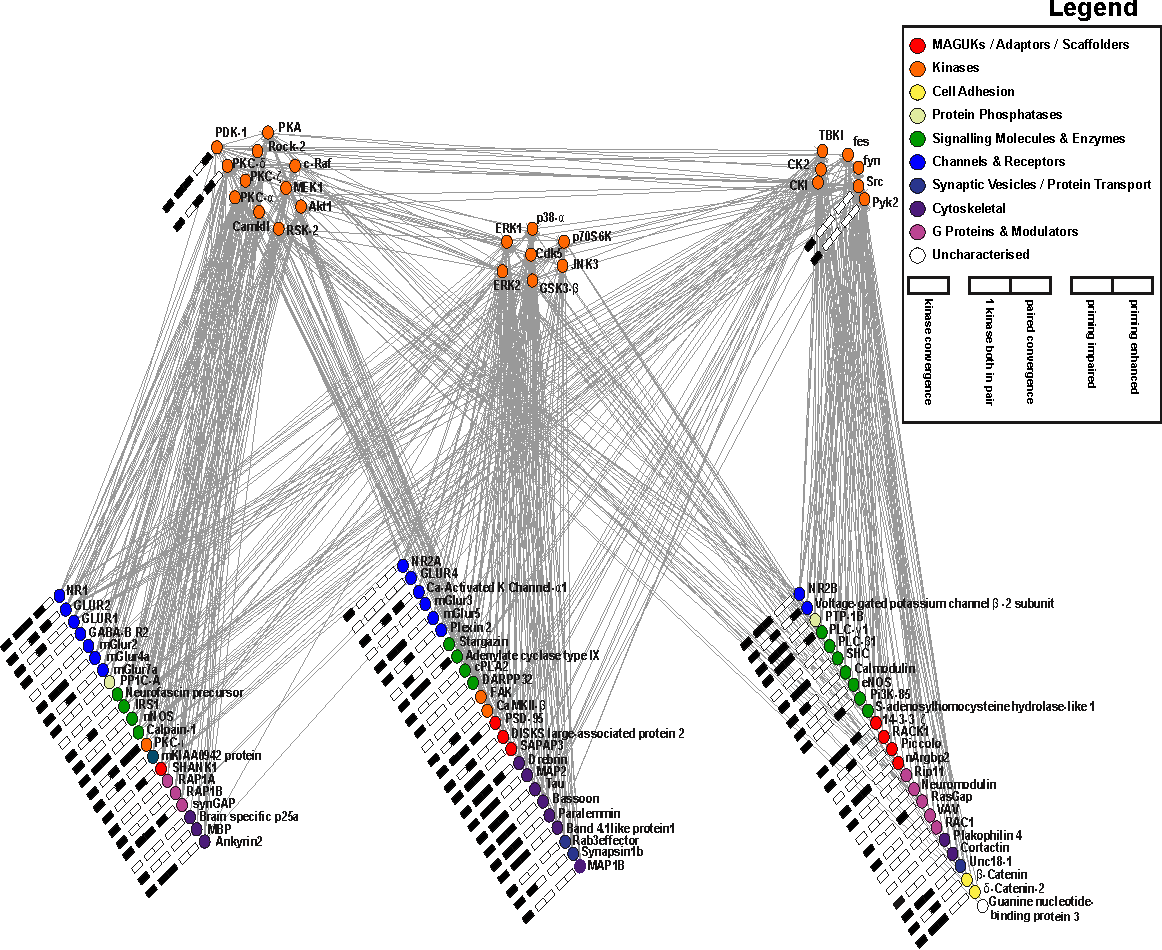
\includegraphics[width=15cm]{2000102CobaFig4.pdf}

 \citerr{Coba2009phosphorylation}
\end{minipage}
 \begin{minipage}[b]{10cm}
 In reality, a synapse is a complex dynamical system.

 \vp We will describe a synapse by a stochastic process with a finite number of states, $n$.

 \vp Potentiation and depression cause transitions between these states.
\end{minipage}
 \vp
\parbox[c]{25cm}{
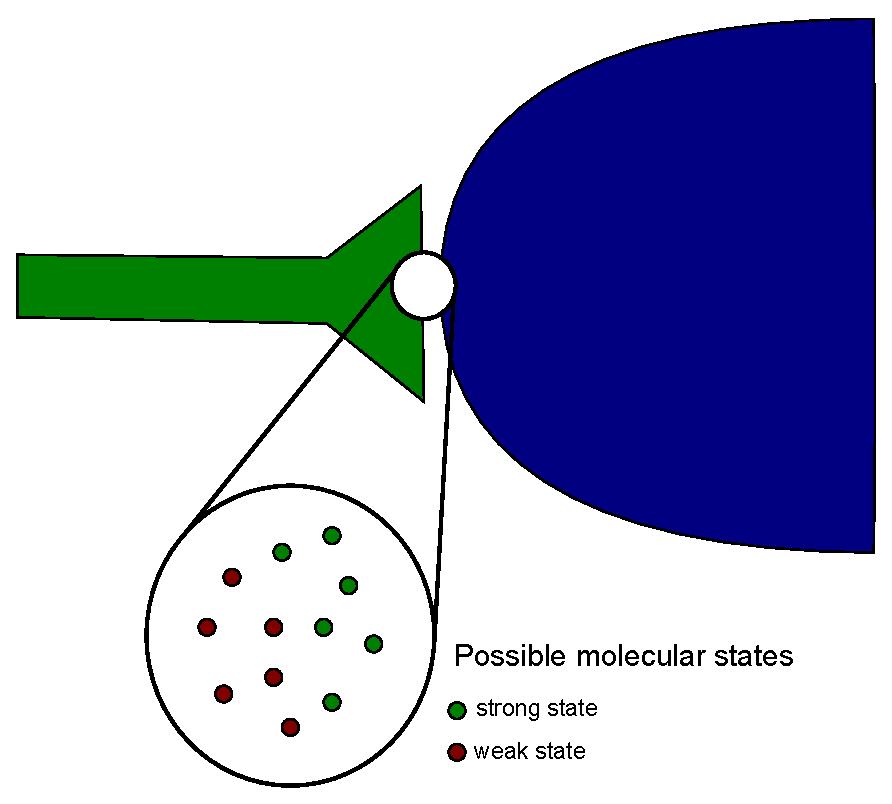
\includegraphics[width=9cm]{synapse.eps}
\hfill%\hspace{3cm}
 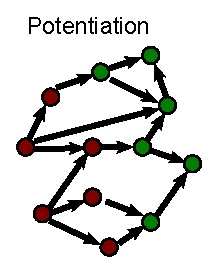
\includegraphics[width=3cm]{pot.eps}
 \hspace{2cm}
 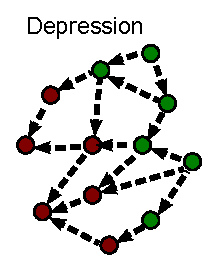
\includegraphics[width=3cm]{dep.eps}
}
%
\end{block}

%-------------Box--------------------------------------------------------

\begin{block}{Cascade and multistate models}
%
 Two example models of metaplasticity in complex synapses.
 \begin{center}
 \parbox[t]{30cm}{
 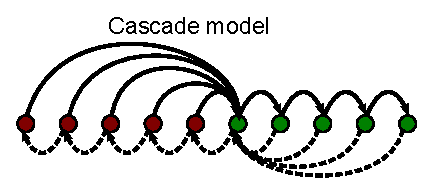
\includegraphics[width=12cm]{cascade.eps}
 \hspace{2cm}
 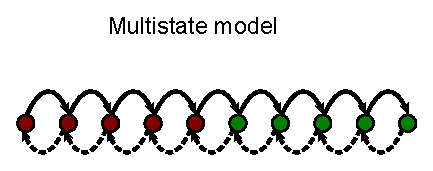
\includegraphics[width=12cm]{multistate.eps}
 }
 \end{center}
 \citerr{Fusi2005cascade,Fusi2007multistate}

 These have different memory storage properties
 \begin{center}
 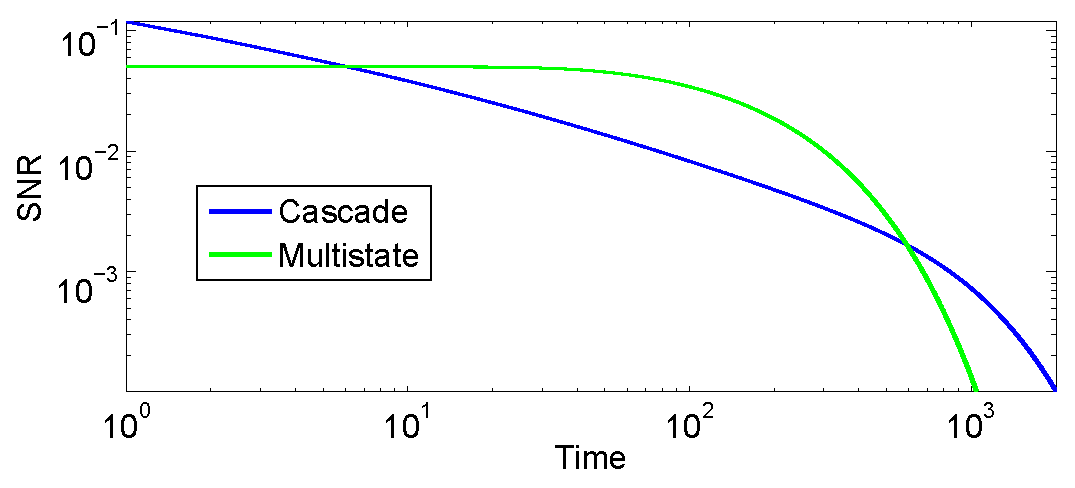
\includegraphics[width=15cm]{cascms.eps}
 \end{center}
%
\end{block}


%-------------Box--------------------------------------------------------

\begin{block}{Questions}
%
 \begin{itemize}
   \item How is structure of \net related to function?
   \item What are the upper bounds on different measures of memory?
   \item Which \net topologies maximize these measures?
 \end{itemize}
%
\end{block}


%-------------Column--------------------------------------------------------
\end{column}

%-------------Column--------------------------------------------------------
\begin{column}{0.37\linewidth}

\section{Framework}

%-------------Box--------------------------------------------------------

\begin{block}{Metaplasticity models}
%
 We have $N$ synapses with $n$ internal states.

 We have two Markov processes describing transition probabilities for potentiation, $\M\pot$, and depression, $\M\dep$.

 \vp Plasticity events are potentiating with probability $f\pot$ and depressing with probability $f\dep$.

 \vp After the memory we are tracking, subsequent plasticity events occur at rate $r$, with transition probabilities
 %
 \begin{equation*}
   \M\frg = f\pot\M\pot + f\dep\M\dep.
 \end{equation*}
 %
 This will eventually return it to the equilibrium distribution, $\eq$.
%
\end{block}

%-------------Box--------------------------------------------------------

\begin{block}{Memory curve}
%
 We use the ideal observer approach: read synaptic weights directly.
 This is an upper bound on what could be read from network activity.

 Reconstruction probability of a single synapse:
 %
 \begin{equation*}
   s(t) = f\pot P(\text{strong},t|\text{pot},0) + f\dep P(\text{weak},t|\text{dep},0)
 \end{equation*}
 %
 Alternatively, if $\W$ is an $N$-element vector of synaptic strengths,
 %
 \begin{equation*}
   \begin{aligned}
     \text{Signal} &= \av{\W_\text{ideal} \cdot \W(t) -  \W_\text{ideal} \cdot \W(\infty)}\\
     \text{Noise} &= \var\prn{\W_\text{ideal} \cdot \W(\infty)}
   \end{aligned}
 \end{equation*}
 %
 If we ignore correlations between different synapses, signal-to-noise ratio:
 %
 \begin{equation*}
   \SNR(t) \sim \sqrt{N}(s(t)-s(\infty)).
 \end{equation*}
 %
%
\end{block}


\section{Upper bounds on performance}

%-------------Box--------------------------------------------------------

\begin{block}{Area bound}
%
\parbox[c]{20cm}{
 We can show that the area under the SNR curve is bounded:
 %
 \begin{equation*}
   A \leq \sqrt{N}(n-1)/r.
 \end{equation*}
 %
 This leads to a bound on the lifetime of a memory:\\
 %
 \begin{equation*}
 \begin{aligned}
   \SNR(\text{lifetime})&=1
   &\qquad
   \implies
   \quad
   \text{lifetime} &< A.
 \end{aligned}
 \end{equation*}
 %
}
\hfill
\parbox[c]{16cm}{
 %
 \begin{center}
   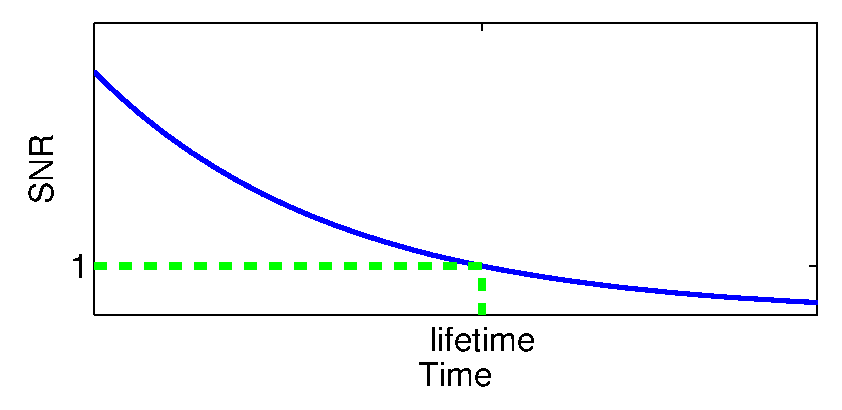
\includegraphics[width=15cm]{lifetime.eps}
 \end{center}
 %
}

 This is saturated by a \net with the multistate topology.
%
\end{block}

%-------------Box--------------------------------------------------------

\begin{block}{Ordering the states}
%
 Let $\fpt_{ij}$ be the mean first passage time from sate $i$ to state $j$.
 The following quantity
 %
 \begin{equation*}
   \eta = \sum_j \fpt_{ij} \eq_j,
 \end{equation*}
 %
 is independent of the initial state $i$.
 It is known as Kemeney's constant. \citerr{kemeny1960finite}

 \vp We define:
 %
 \begin{equation*}
   \eta^+_i = \sum_{j\in\text{strong}} \fpt_{ij} \eq_j,
   \qquad
   \eta^-_i = \sum_{j\in\text{weak}} \fpt_{ij} \eq_j.
 \end{equation*}
 %
 These measure ``distance'' to the srong/weak states.
 They can be used to put the states in order (increasing $\eta^-$ or decreasing $\eta^+$).
%
\end{block}

%-------------Box--------------------------------------------------------

\begin{block}{Maximal area}
%
 Given any \net, we can construct one with the multistate topology that has
\parbox[c]{15cm}{
 \begin{itemize}
   \item same state order,
   \item same equilibrium distribution,
   \item larger area.
 \end{itemize}
}
\parbox[c]{15cm}{
 %
 \begin{center}
   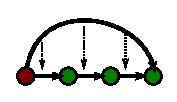
\includegraphics[width=6cm]{shortcut.eps}
 \end{center}
 %
}

 Uses a deformation that reduces ``shortcut'' transition probabilities and increases the bypassed ``direct'' ones.

 \vp The area of this model is
 %
 \begin{equation*}
   A = \frac{2\sqrt{N}}{r}\sum_k \eq_k \abs{k-\av{k}}.
 \end{equation*}
 %
 Maximum is when all probability is at ends.
%
\end{block}





%-------------Column--------------------------------------------------------
\end{column}

%-------------Column--------------------------------------------------------
\begin{column}{0.32\linewidth}



\section{Envelope memory curve}


%-------------Box--------------------------------------------------------

\begin{block}{Maximal SNR curve}
%
 Markov process $\implies$ SNR is sum of exponentials.

 \vp If we find the maximum sum of exponentials \alert{at one time} subject to upper bounds on initial SNR and area,
 we get an upper bound on SNR at that time.

 \vp Resulting curve is always a single exponential.

 \vp If we vary the time at which we find the optimum, we get an envelope curve with a power law tail.
 \begin{center}
 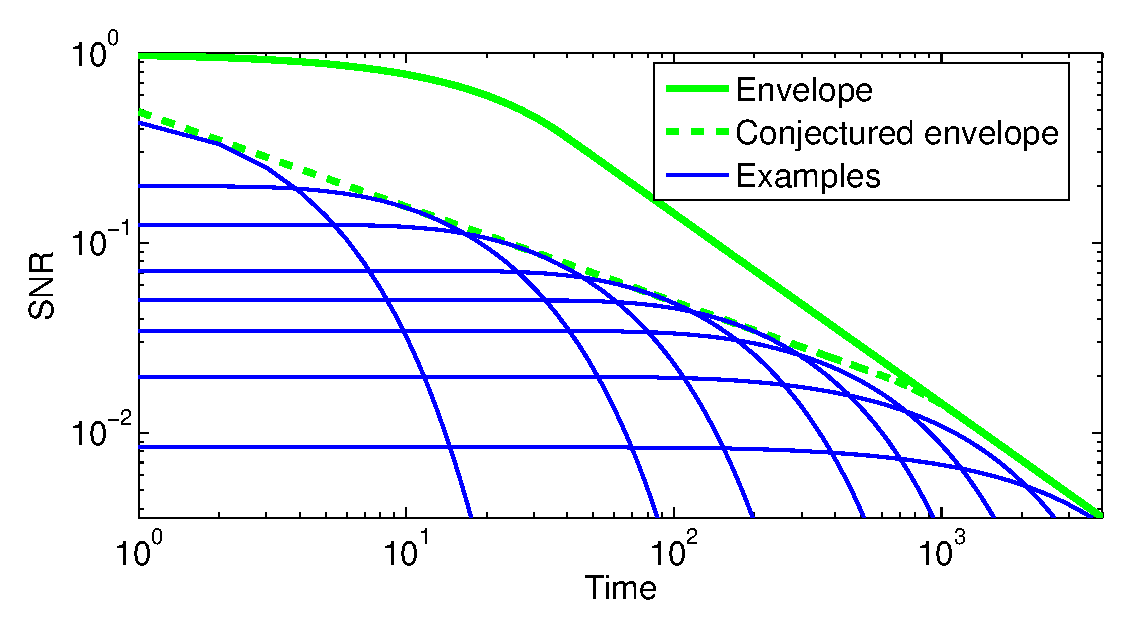
\includegraphics[width=15cm]{env.eps}
 \end{center}
%
\end{block}

%-------------Box--------------------------------------------------------

\begin{block}{Extra constraint}
%
 The envelope above may not be tight.

 \vp We can get a tight envelope
 -- one that can be saturated at any single time by some model --
 if we add one more constraint.

 \vp Schematically, mode by mode:
 %
 \begin{equation*}
   \SNR(0)\sqrt{\text{time-scale}} \leq \sqrt{N}\cdot \CO(1).
 \end{equation*}
 %
 We have found no model can exceed this. It is saturated by a diffusive chain:
 %
 \begin{equation*}
   \SNR(0) \sim \frac{1}{n},
   \qquad
   \text{time-scale} \sim n^2.
 \end{equation*}
 %
%
\end{block}

%-------------Box--------------------------------------------------------

\begin{block}{Maximum lifetime}
%
 We can use the envelope to get a stricter bound on the lifetime of a memory
 %
 \begin{equation*}
 \begin{aligned}
   \operatorname{Envelope}(\text{max lifetime}) = 1, \qquad
   \text{max lifetime}  = \frac{\sqrt{N}(n-1)}{\e r}.
 \end{aligned}
 \end{equation*}
 %
%
\end{block}

%-------------Box--------------------------------------------------------

\begin{block}{References}
%
 {\small
 \bibliographystyle{unsrt_poster}
 \bibliography{neuro,maths}
 }
%
\end{block}


\end{column}




%%%%%%%%%%%%%%%%%%%%%%%%%%%%%%%%%%%%%%%%%%%%%%%%%%%%%%%%%%%%%%%%%%%%%%%%%%%
%-----End----------------------------------------------------------------

\end{columns}

\end{frame}

\end{document}
